\documentclass{sig-alternate}

\begin{document}

\conferenceinfo{Heptinstall}{'13 Aberystwyth University}

\title{{\ttlit CS21120 Assignment 2:} Data Structures and Algorithm Analysis
Paper
}

\numberofauthors{1} 

\author{
\alignauthor
Craig Heptinstall- 01/05/2013\\
       \affaddr{Software Engineering Student}\\
       \affaddr{Department of Computer Science}\\
       \affaddr{Aberystwyth University, Aberystwyth}\\
       \email{crh13@aber.ac.uk}
       \date{01/05/2013}
}
\crdata{01/05/13}
\CopyrightYear{2013}
\maketitle
\begin{abstract}
This paper provides my solution to research into different scheduling
algorithms present in day to day systems just as in  a CPU. I wanted to look
into the different methods of scheduling processes in the most efficient ways
possible, taking into account the size of processes, time and priority. This
paper will explore a range of different algorithms to help solve my question in
finding the most efficient and suitable in the data I will provide. To ensure
more precision amongst my results I ensured a good number of tests were
implemented on each of the algorithms by means of using different sets of data
concerning size, priority and amount of processes. 

I have also compared each algorithm concerning each set of results to see where
some scheduling methods work better than others and where each algorithm
provides strengths or weaknesses to a situation against other possible
schedulers. In all, although I found that some schedulers worked better than
others across a wider range of situations, a key finding was that there is
never one true answer to the best scheduler and this adds to the problem of
finding the most efficient as possible across systems. This research has taught
me much about the convenience of using different schedulers for different
situations which I hope to detail in this report.
\end{abstract}

\category{Data Structures and Algorithms}{Scheduling algorithms}[processes]

\category{Software Engineering}{Algorithms}[complexity measures, performance
measures]

\terms{Along with this report, and any of the job files described can be
accessed within the bin folder in the project. 
I have also included testing of the JUnit kind within the project file. A class
diagram is also available in the assignment folder.
This PDF and Tex file can be found in the assignment folder also.
}

\section{Introduction}
To introduce this paper in solution to assignment two for CS21120, I will now
briefly explain the reasons for conducting these tests on scheduling processes. 

Because there is such a vast amount of different scheduling algorithms
available, I wanted to test a discrete set of these and test each of them with
ranges of pieces of data. Each slice of data would be placed into a file
containing a number of processes, each with a name, priority, start time, CPU
cycles and CPU cycles blocked. These would define what the sizes, priorities and
amount of cycles required to complete each process would be. Using my
constructed algorithms, I then would run through this list and test each
scheduler algorithm to see how many cycles to 'CPU' would be required to perform
to complete the entirety of the list. The programming language I have used to
create this algorithms in is Java, which allows easy access to pre-defined
actions such as queues which allowed myself to use this as the basis of waiting
processes.

I must mention that along with code constructed by myself, the
\textit{FirstComeFirstServed} class was already provided as a basis for other
algorithms and that I was merely using code given in the assignment and then
providing additions to create the extra processing functionality. I can confirm
here that I have not modified any of the code provided to me. Again, pieces of
data was also provided to me contain example processes which I have also added
to and created new sets of to ensure maximum test ranges for each of the
scheduling algorithms.
\vspace{3mm}

Below I have listed the set of algorithms I have performed in the piece of
research concerning four scheduling choices:

\begin{itemize}
\item{First Come First Served Scheduler \textit{ - Provided by Richard Shipman}}
\item{Priority Queue Scheduler}
\item{Lottery Scheduler}
\item{Shortest Job First Scheduler}
\end{itemize}

In the following sections of the paper I will detail each scheduler implemented
and show the performance of each under different circumstantial tests. I will
also provide basis for comparisons between each, and use illustrations where
necessary.
\vspace{3mm}

\section{{\secit Scheduling} Algorithms}
For each of the algorithms implemented, I will now take a look at how each
scheduler works, and how each performed with the data sets I provided. I will
also comment on each by saying how I thought they performed, and if they
performed as expected. In some circumstances, I will test the scheduler a number
of times with the same data where necessary to get fair results such as the
Lottery scheduler. 

By looking at each scheduler separately, I will then be able to base my
comparisons on the results of each. As you will see, I will look into great
detail into the way larger sets of data, IO or idle time can affect performance
of each of these algorithms to bring out the strengths and weaknesses out of
each. 

\subsection{First Come First Served}
The first scheduler that was implemented was provided to me with the assignment
brief which was the First come first served algorithm. This algorithm works on
the simple basis that what ever process comes first in the list would be added
to the Job queue first and ultimately ran first until the process was either
completed or blocked for IO. In the case that a process was blocked for IO the
process would allow the IO to complete where required, and then the process
would join the back of the queue. The next Job at the head of the queue would
then run. 
This scheduling algorithm being the simplest takes into no account the priority
or sizes of processes which I believed would damage the length of time taken to
complete the total amount of processes.

Below you will see the first set of runs using the job files presented to me
along with the brief at the start of the assignment:
\begin{table}[!h]
\centering
\caption{FIFO Results Table}
\begin{tabular}{|c|c|c|c|c|} \hline
&a&Test 1&Test 2&Test 3\\ \hline
Mean Process Time&27&48&54&134\\ \hline
Total CPU Time&40&75&69&191\\ \hline
Context Switches&4&10&15&26\\ \hline
Total Idle Time&8&6&0&9\\ \hline
\end{tabular}
\end{table}

Looking at the results of the tests provided for me, and In the first file,
a.jobs contained three different pieces of data to run through. This was that of
two CPU's and then a mixed IO task. In that order of entering the system, when
CPU one was half complete it was blocked for IO, resulting it moving to the back
of the queue. Because of this, the algorithm ensured that the next task would
start now first. All this resulted in CPU two finishing before CPU one because
of the IO and because of the first in the queue rule applied to this algorithm. 

This is where the algorithm does seem to have a flaw, because depending if IO is
involved in the process of the queue, then any interrupted tasks can be disrupted
and then take longer to be completed. To test this theory, I did the same tests
but with a file I created, which was simply a.jobs but in reverse.

 The results can be seen below in table 2:
\vspace{18mm}
\begin{table}[!h]
\centering
\caption{FIFO MyTest1.jobs file}
\begin{tabular}{|c|c|} \hline
&MyTest1.jobs\\ \hline
Mean Process Time&26\\ \hline
Total CPU Time&33\\ \hline
Context Switches&5\\ \hline
Total Idle Time&1\\ \hline
\end{tabular}
\end{table}

From looking at results in the test file I created, by swapping around tasks the
Total CPU time did drop because now the IO was first in queue. This meant less
distribution time of the other tasks, as you will see in the drop in average time
to process a task. Idle time has also dropped because of this. In this example,
CPU2 was placed higher in the file than CPU1 and successfully completed before
CPU1 because I placed IO at the top. This result helps show the importance of IO
tasks when looking at this algorithm. 

To show this even further, I made a second file to tests this scheduler with,
containing only processes and no IO. starting from CPU1 through 3, I ran the
program and as expected the completed list of tasks were in the order as they
were added. Each had the same amount of cpu cycles as CPU2 from previous files,
and the same priority. The order of the output is compared below:

\begin{table}[!h]
\centering
\caption{Comparison Of Ordered Results}
\begin{tabular}{|c|c|c|} \hline
Test File&Order In&Order Out\\ \hline
a.jobs&CPU1,CPU2,Test(IO)&CPU2,CPU1,Test(IO)\\ \hline
MyTest1.jobs&Test(IO),CPU2, CPU1&CPU2,Test(IO),CPU1\\ \hline
MyTest2.jobs&CPU1,CPU2,CPU3&CPU1,CPU2,CPU3\\ \hline
\end{tabular}
\end{table}

All the Job files associated with these tests can be found in the bin folder of
the project containing the different schedulers.

\subsection{Priority Queue}
As the second scheduler, I chose to implement this based around the first in
first out alternative, yet with the addition of checking the priority of a
process before assigning it next in the job queue. This meant that anything with
a higher priority in a day to day system would get more attention from the CPU,
and complete before less important tasks. I felt this as a good way of
scheduling tasks because even if the total CPU time was slower than another
scheduler, at least the more important tasks would be completed before other
tasks unlike in other schedulers that would go for pure total CPU speed. 
\vspace{3mm}
Again, I conducted tests on this scheduler using the same test jobs as I used
for the previous algorithm yet with some additions and changes to ensure more
precision and flexibility about my results. The results for the standard tests
are as follows:
\begin{table}[!h]
\centering
\caption{Priority Queue Results Table}
\begin{tabular}{|c|c|c|c|c|} \hline
&a&Test 1&Test 2&Test 3\\ \hline
Mean Process Time&30&46&45&118\\ \hline
Total CPU Time&52&69&69&182\\ \hline
Context Switches&6&14&16&35\\ \hline
Total Idle Time&20&0&0&0\\ \hline
\end{tabular}
\end{table}

\vspace{5mm}

Looking at the results from the priority queue algorithm results in table 4, I
have noticed that priority queue seems to work better as the amount of processes
and process time is required. For instance, a good number of processes would
work best with this algorithm because this algorithm looks to complete the most
important tasks before others clearing space for less needed processes. This
seems to give the illusion of pre-defining what processes are to be run in what
order to ensure the system delivers good efficiency. You will notice that the
idle time drops as the amount of processes increases, proving my point further.
This simple graph shows what happens between the correlation of process time and
idle time:

\begin{figure}[!h]
\centering
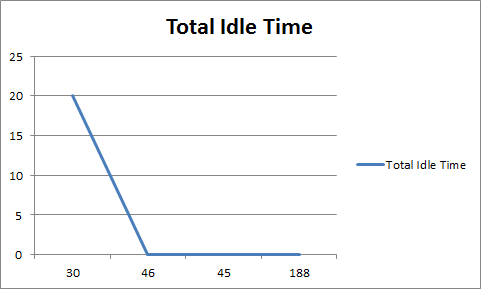
\includegraphics[scale=0.6]{images/priority1.png}
\caption{Using the test files, this shows CPU Total ticks (X axis) plotted
against the total Idle time (Y axis).}
\end{figure}

 Because this algorithm always sorts by priority, I wanted to look at what would
occur if for instance all the processes had the same priority.  Again, I have
created my own file to test (MyTest3.jobs) with and shown the results below:

\begin{table}[!h]
\centering
\caption{Priority Queue Results Table}
\begin{tabular}{|c|c|c|} \hline
&Test3.jobs&Test.jobs(original)\\ \hline
Mean Process Time&48&46\\ \hline
Total CPU Time&75&69\\ \hline
Context Switches&10&14\\ \hline
Total Idle Time&6&0\\ \hline
\end{tabular}
\end{table}

The file I used to test shown above was a template based from Test.jobs given to
me in the brief but where all the priorities had been changed to 1. As you will
see, in the test file before the priorities had been changed, the test processes
run faster and had better statistics all round than my modified version. This
shows that if a set of processes do not have defined priorities, this algorithm
could have problems. Whilst on the other hand, if priorities are defined, it
seems to handle larger tasks better the bigger they are.

\subsection{Lottery}
For my second self-implemented scheduler, I wanted to try an algorithm that did
not take into consideration and of the attributes of any jobs in the files, that
simply chose at random which job would next be processed. This was done by
easily getting a random number from zero to the amount of processes left minus
one using the util class in Java and then using this as the head of the queue.
By repeating this after every process, it ensured that the order of processes
was always random and therefore would affect the results for better and for
worse.

 Because of this, I firstly ensured that I would have to test the algorithm many
times for each of the job files. To do this, I ran each job file in a loop
around a thousand times and then used the averages of each piece of data as a
basis of result for this scheduler.

I must note here that the way I implemented this algorithm was slightly different
to that shown on numerous sites across the web such as in the Wikipedia-lottery
scheduler page in the sense that usually a bigger task would
get more 'lottery tickets'. In my opinion, having simply one ticket per process
would generally work in the same way over a matter of time, this is because if a
task had three times more tickets than another, the odds would say for every
three times the bigger process is chosen, the smaller one would. My method
simply allows any process to have the same chance, but instead some processes my
finish earlier, allowing others much higher chance. This would eventually even
out the odds.
\vspace{3mm}

As an example of this testing to show the randomness of the Lottery scheduler, I
have created a graph below showing the results of this scheduler after being run
100 times on Test.jobs. I have also shown the average on this graph:
\begin{figure}[!h]
\centering
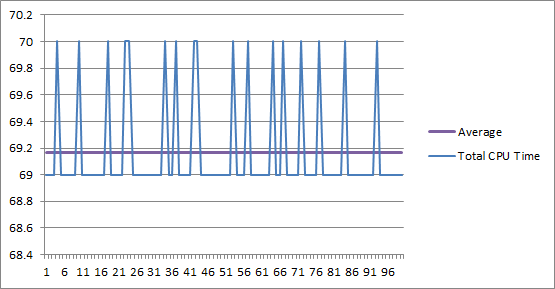
\includegraphics[scale=0.6]{images/lottery1.png}
\caption{Using the a.jobs file, one hundred tests (X axis) plotted against the
total CPU ticks per run(Y axis).}
\end{figure}

And using the standard test job files, with averages I have completed the
standard tests for each of the job files given to me in this assignment:
\begin{table}[!h]
\centering
\caption{Lottery Results Table}
\begin{tabular}{|c|c|c|c|c|} \hline
&a&Test 1&Test 2&Test 3\\ \hline
Mean Process Time&25&56&62&142\\ \hline
Total CPU Time&32&69&69&182\\ \hline
Context Switches&9&42&43&129\\ \hline
Total Idle Time&0&0&0&0\\ \hline
\end{tabular}
\end{table}

As you can see, even with random processes being chosen, the example file I
selected showed that generally the scheduler dealt with the processing at quite
a steady rate. Although It may be reliable on small sets of data because the
choices for processes are lesser than others, with a large number of process,
this could become unreliable. To test this, I created a test job file containing
lots of processes, and again tested this many times. The graph of the amount of
total ticks is shown below:

\begin{figure}[!h]
\centering
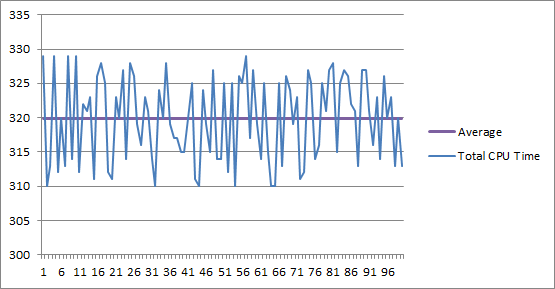
\includegraphics[scale=0.6]{images/lottery2.png}
\caption{Using the Test4.jobs file (containing lots of processes), one hundred
tests (X axis) plotted against the total CPU ticks per run(Y axis).}
\end{figure}

Where I did use larger data sets, the difference increases between the amount of
ticks, making the lottery scheduler more ideal for smaller process amounts.
Where a large system used this scheduler, the system could experience fast and
slow speeds at random.

\subsection{Shortest Job First}
For the final of the algorithms implemented in this paper, the Shortest job
first schedule was one that I believed would work well under a good amount of
circumstances. For instance, where there are lots of smaller tasks in length,
this algorithm would work well in the sense that these tasks would be completed
first, meaning the majority of jobs would be complete leaving only those that
are larger. Therefore I will be looking at testing the weaknesses of this later
on by only giving the system big/ long processes to run through. This algorithm,
as stated in the name looks through the processes, each time deducting the ticks
of the CPU used on the process from the total length of the process. The
remainder is then compared amongst all of the processes and the one with the
least remaining is run. 

This algorithm I think was much more interesting to test because of the way it
selected processes and by mixing different length processes around I could see
the affects of speed and manner which It chose different processes.

\vspace{3mm}
Alike the previous three, I began by firstly testing the jobs given to me in the
brief:
\begin{table}[!h]
\centering
\caption{Shortest Job First Results Table}
\begin{tabular}{|c|c|c|c|c|} \hline
&a&Test 1&Test 2&Test 3\\ \hline
Mean Process Time&29&43&44&90\\ \hline
Total CPU Time&52&81&82&182\\ \hline
Context Switches&5&11&18&39\\ \hline
Total Idle Time&20&12&13&0\\ \hline
\end{tabular}
\end{table}

With this scheduler, I noticed that a great deal of context switched and idle
time seemed to accumulate when bigger lists of data were being processed. My
explanation for this would be because of the way the algorithm works means that
when there are a lot of processes with the same length, it must change between
them all when a shorter task is detected. Generally though, this is similar to
the priority queue scheduler in the sense that the larger the amount of
processes, the better the scheduler would work. Another issue with this though
would be that although more tasks would be complete because shorter ones would
be first, any more important larger tasks would be left until the end. This is
not always ideal in some systems.

In my test job file for this scheduler, I tested what happens to higher priority
tasks when they are larger, and when lower priority processes are smaller:

\vspace{3mm}
\textit{MyTest5.jobs:}
\begin{itemize}
\item{CPU1-Priority 1, Size: 15}
\item{CPU2-Priority 2, Size: 10}
\item{CPU3-Priority 3, Size: 5}
\end{itemize}
The order they completed in: CPU3, CPU2, CPU1.

This is because the shortest also has the lowest priority resulting in this
algorithm not being ideal for this situation. Again, any of the test files
created by myself can be found within the bin folder under the Java project.

\section{Comparisons of Schedulers}
Now that I have completed looking in detail at each of the different schedulers
separately, I will now look at them all as a group, showing what I discovered in
terms of difference in speed and the way that each handled prioritising each
process for a number of jobs.

 To do this successfully, I am going to use a range of graphs and charts showing
the differences in performances, and highlight which algorithms work better
under different circumstances. At the end of this section I will give a brief
summary of each algorithm and say which I believed did the best at certain
processing than others. 
\vspace{3mm}

Firstly, to look at and compare how each scheduler performed at the four basic
job routines, I have shown the comparisons below in a set of tables:
\begin{table}[!h]
\centering
\caption{a.jobs File Comparison}
\begin{tabular}{|c|c|c|c|c|c|} \hline
&FIFO&Priority&Lottery&Shortest F.\\ \hline
Mean Process T.&27&30&25&29\\ \hline
Total CPU Time&40&52&32&52\\ \hline
Context Sw.&4&6&9&5\\ \hline
Total Idle Time&8&20&0&20\\ \hline
\end{tabular}
\end{table}

As you can see in the above table, the lottery scheduler performed best here in
most categories, although did come last at context switches. Because the lottery
algorithm has managed to spread out the processing fairly due to the random
choices, it has meant that a lot of switching processes has taken place. 

The priority queue has not performed well alike my expectations of it, being
that having only three priorities does not suffice for the algorithm to be
greatly affective. This has resulted in a lot of processing time for each task,
therefore a lot of idle time. First in first out managed the processing well,
although did not match that of the lottery, because of the IO which interrupted
some processing resulting in moving processes to the back of the queue. Finally,
the shortest first algorithm managed to keep the processing time relatively low,
but suffered in the lack of processes, meaning it almost acted like a priority
queue.
\vspace{3mm}

Similarly with the second Jobs file:

\begin{table}[!h]
\centering
\caption{Test.jobs File Comparison}
\begin{tabular}{|c|c|c|c|c|c|} \hline
&FIFO&Priority&Lottery&Shortest F.\\ \hline
Mean Process T.&48&46&56&43\\ \hline
Total CPU Time&75&69&69&81\\ \hline
Context Sw.&10&14&42&11\\ \hline
Total Idle Time&6&0&0&12\\ \hline
\end{tabular}
\end{table}

Testing all four with the second standard test file shows that now the data
amount is getting larger, the priority queue performs much better. This time,
the priority queue has the best record for both total time and mean time for
processing. This is because the larger amount of processes now are affected much
more by priorities and act quicker this way than simply running through the list
like first in first out would.

 The lottery algorithm is almost on par with the priority schedule here but is
not as strong in terms of context switching which will have affected its
performance greatly because of the many random choices. The shortest first
scheduler performed disappointingly because of the total time used by the CPU.
This is due to idle time and total amounts of CPU on processes used due to it
getting through smaller ones first but then leaving larger ones until last.
\vspace{3mm}

And with the final file, skipping Test2.jobs because of its similarity of
aspects to test 1:

\begin{table}[!h]
\centering
\caption{Test3.jobs File Comparison}
\begin{tabular}{|c|c|c|c|c|c|} \hline
&FIFO&Priority&Lottery&Shortest F.\\ \hline
Mean Process T.&134&118&142&90\\ \hline
Total CPU Time&191&182&182&182\\ \hline
Context Sw.&26&35&129&39\\ \hline
Total Idle Time&9&0&0&0\\ \hline
\end{tabular}
\end{table}

This highlights the longer tests performed on each algorithm and shows the
strengths of the priority and shortest first algorithms. Where the Total CPU
time is concerned all algorithms steady out to roughly the same level here, yet
when looking at the mean process time and context switches/ idle time, shortest
first and priority act much more efficiently because of the larger amount of
processes in the file. 

The first in fist out algorithm takes exceptionally long to complete the total
job, whilst the lottery algorithm performs equally poorly due the amount of
required context switches. For large files, the lottery algorithm would have to
randomly choose from any of a massive amount of processes each time resulting in
more chance of a blocked process for IO.
\vspace{3mm}

Now that I have completed comparing using standard tests along with information
I have learned from looking at each scheduler individually, I will now show using
graphs, how each compare under certain circumstances. 

Starting with how the larger the amount of processes affects the total time of
the CPU taken. This incorporates a number of different jobs that I have
performed in this paper. This is shown in figure 4.

\begin{figure}[!h]
\centering
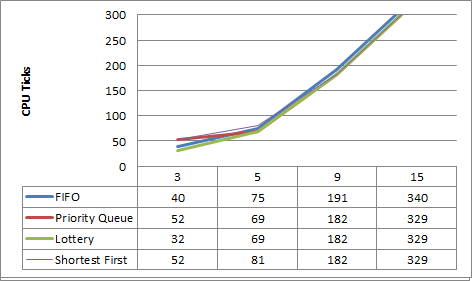
\includegraphics[scale=0.6]{images/compare1.png}
\caption{X Axis(number of processes) against Y Axis (total time of CPU)}
\end{figure}

As you can see, although the graph does not show a massive difference in some
values, any change in the amount of ticks between them can make considerable
difference in large systems. the best performing ones at smaller tasks tend not
be be the best at larger tasks. For instance, from looking back in this paper
and looking at the statistics of the first in first out and the lottery
algorithms, these both have good speeds in terms of total CPU time when the
tasks are smaller; up to five and then the other two algorithms work best. 

I think this was due to the way each algorithm worked, first in first out must
loop through the queue many times when there is IO, while the lottery has much
more processes to pick at random from.

\vspace{3mm}
I have also constructed an average context switch bar chart below, showing the
difference in the amount of times on average each algorithm performs when
changing from one process to another. This is a key part of the scheduling
process to look at, because it can reflect which algorithm s are spreading out
the processing time and which follow more direct routes.

\begin{figure}[!h]
\centering
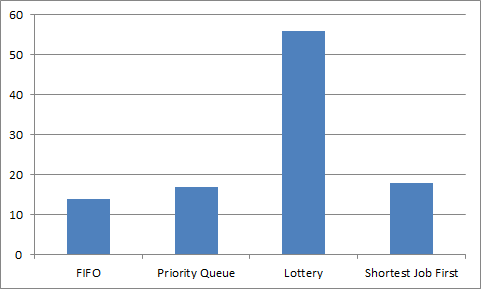
\includegraphics[scale=0.6]{images/compare2.png}
\caption{Number of switches on average for all of the job files implemented in
this paper.}
\end{figure}

As seen upon the bar chart, the lottery algorithm performs up to four times as
many switches on average to the others. This is simply explained again by the
random choosing of a different process after each click of the CPU. other
algorithms such as the priority queue and shortest first do reasonably well at
keeping down the switches because the choices are made repeatedly on priority
and size of the processes which should not change. As for the FIFO algorithm, I
expected this to be best at this because of the simple way it stays at a process
until IO is called or a process is complete which requires less switches.

\section{Conclusions}
In this brief summary, I will now describe my overall findings after writing and
testing each of the algorithms/ schedulers. Firstly, if I had to state which
algorithms worked best overall, I could not give a definitive answer to this, but
instead provide a range of answers. 

For instance, through testing the first in first out and lottery schedulers, I
found these worked better with smaller chunks of processes to handle. When it
came to larger chunks, the priority and shortest time remaining schedulers
preformed much better. This shows that the answer depends on the needs of the
system at the time, although the lottery scheduler has good all round
performance bar the switches data.

I could have explored further algorithms in this paper such as round robin but
chose to stick to ones which were implemented more differently to get a wider
scope of ways to schedule data.

Along with learning a great deal of how day to day schedulers work in a range
off systems, I have also gained good experience in the use of analszing such
data as from the scheduling of tasks, in understanding what the data means and
what affects changing data and the algorithms themselves can do. 

If I were to complete a similar project to this one again, using my new found
knowledge I would have liked to implement a wider set of schedulers, such as
the 'completely fair scheduler', round robin or other alternatives. This would
allow me to grasp a greater understanding of how processes in systems are
carried out.

\subsection{Executive Summary}
In this final section acting as an account of the entire project but in great
briefness, I will look back over the project and give an account of my actions.

Upon being given the assignment, the first and most important task was learning 
how the existing code functioned, for instance how data was sent to and from the
different scheduling algorithms. I also had to understand the properties files
which allowed me to insert my own scheduling classes to the project.

Once this had been completed, and I had selected and implemented my schedulers,
I then ran some dummy tests with the standard job files that had been presented
to me in the bin folder of the project. These tests simply allowed me to try my
new schedulers to see if they functioned as planned. I did come across an issue
with the lottery scheduler that made the random set of numbers the same on every
run. This was solved after I found out about the '.seed' function that I then
set to the current time in order to make the random processes chosen each time
different.

After the initial tests, I then looked at the data given in the brief and
tested each 'job' file on each scheduler. Along with this, I described how each
algorithm worked and my overall opinion of its performance. 

To back up my research into each one, I wrote my own job files where necessary
to exploit any weaknesses or strengths such as in the priority queue scheduler
where I created a job file with although some smaller tasks would normally be
completed fairly quickly, this did not happen because of their low priorities. 

Along with thee testing of each, I also created graphs where necessary, such as
in the lottery algorithm where I needed to show the reliability levels of the
scheduler which showed that the level of stability decreased as the number of
processes became larger.

After each of the individual tests, I then went to compare them all together in
terms of how each handled certain systems, number of switches between processes,
and most importantly the raw speed. In my results I saw that each algorithm did
have its own issues and problems under different stresses.

In so I decided that although the brief did not ask for the best algorithm to be
defined, I would not be able to state one any way. This was because the system
and processable data amounts defines the algorithm that should be used in that
situation. In a larger system, the priority queue and shortest first acted much
better than the others, whilst this was the opposite when it came to the
shortest of the tasks.
\end{document}
